\chapter{La gestion des points}

\section{La capture de points sous Android}
Sous Android, la localisation d'un appareil utilisant une puce GPS est rendue possible. Bien évidemment, plus la puce est performante plus la localisation de l’appareil sera aisée. La capture de points se fait grâce à trois fournisseurs (\textit{providers}) différents.

\subsection{Les \textit{providers}}
Nous parlerons ici uniquement des providers nécessaire au fonctionnement de notre application à savoir le \textit{NETWORK\_PROVIDER} et \textit{GPS\_PROVIDER} cependant un récapitulatif des providers est disponible à l'Annexe \ref{Annexe3}.

\subsubsection{Le \textit{NETWORK\_PROVIDER}}
Ce fournisseur détermine la position du l'appareil en fonction des antennes téléphoniques et des points d'accès au Wi-fi. Il a une précision d'environ 60 mètres. Mais fournis des points beaucoup plus rapidement que le GPS. Nous l'utilisons dans notre application le temps que la puce se synchronise avec le GPS.

\subsubsection{Le \textit{GPS\_PROVIDER}}
De tous les fournisseurs, celui-ci est de loin de plus précis puisqu'il permet de localiser un appareil avec une précision de 6 mètres. Malheureusement, pour se faire, la puce de l'appareil doit se connectée à un GPS est cela peut prendre beaucoup de temps. De plus, tant l'acquisition n'a pas été établie, aucun point ne sera fourni.

\begin{note}
L'utilisation du service de localisation sous Android nécessite des permissions que l'on doit ajouter au \textit{manifest} (Partie \ref{manifest}).
\end{note}

\subsection{Le LocationManager}
\label{locationManager}
Le \verb!LocationManager! représente le service de gestion de capture de points. C'est grâce à cette classe que la localisation de point peut se faire. Son fonctionnement est brièvement représenté par le diagramme \ref{Diagramme Location Manager}. Son instanciation se fait grâce aux services Android. Une fois l'instance obtenue, l'appel à la méthode \verb!requestLocationUpdates! doit être fait en précisant le \textit{provider} utilisé ainsi que deux variables et un \verb!LocationListener!. Les deux variables correspondent au minimum de temps et de distance nécessaire avant la capture d'un nouveau point. La valeur de ces variables est inversement proportionnelle à la consommation de la batterie. A chaque fois qu'un nouveau point est trouvé, le \verb!LocationListener!, qui écoute l'arrivée d'une nouvelle \verb!Location!, va pouvoir l'ajouter  à la liste des points du trajet. C'est également le \verb!LocationListener! qui va vérifier la bonne continuité du signal. En cas de modification, de perte ou de récupération du signal, un appel est effectué via les méthodes correspondantes.

\begin{img}  
	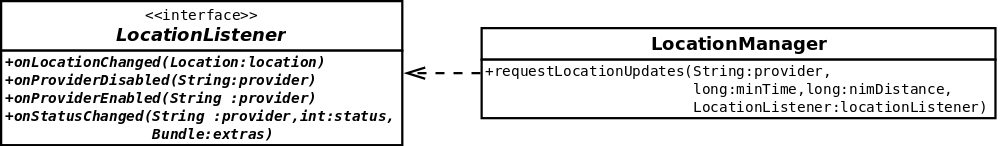
\includegraphics[scale=0.65]{img/LocationManager.png}
	\caption{Fonctionnement du Location Manager}
	\label{Diagramme Location Manager}
\end{img}

\section{Projection d'un point}
Dans la partie précédente, nous avons vu que la capture de points n'est pas très précise. En effet, pour deux trajets réalisés sur le même parcours, on peut avoir des points situés à des endroits différents et pris à des dates différentes. La figure \ref{Représentation des trajets} représente cet écart lors de la capture des points. Afin de pouvoir comparer deux trajets, nous devons projeter les points (ici le point $A$) du trajet réalisé ($t_2$) sur le trajet de référence ($t_1$). Pour cela nous devons calculer les coordonnées du point $H$ pour déterminer le rapport entre $[BH]$ et $[CH]$ et permettre une estimation sur le temps établit pour atteindre le point $A$ sur le trajet $t_1$. Nous pourrons ainsi comparer les temps mis pour atteindre les points $A$ sur $t_2$ et $H$ sur $t_1$.

\begin{img}  
	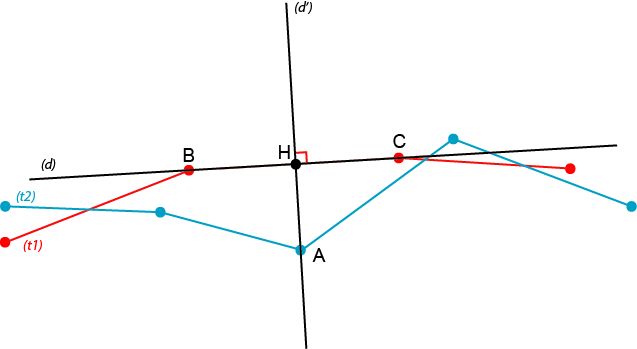
\includegraphics[scale=1]{img/Trajet.png}
	\caption{Représentation des trajets}
	\label{Représentation des trajets}
\end{img}

\subsection{Calcul des coordonnées de H}
On pose trois points $ A(x_a,y_a) $, $ B(x_b,y_b) $ et $ C(x_c,y_c) $ et nous cherchons à calculer les coordonnées de $ H(x_h,y_h) $ (Figure \ref{Représentation des trajets}).
Pour ce faire, nous devons commencer par calculer l'équation de la droite $ d $ passant par les points $B$ et $C$.
On pose donc : 
\[
 	d(x) = mx + n
\]
On cherche à déterminer le coefficient directeur de la droite ($m$). Comme $B \in d$ et $C \in d$, on a :
\[
   m =  \frac{x_b-x_c}{y_b-y_c}
\]
Comme le point $B \in (d)$, il résout l'équation :
\[
   y_b = mx_b + n \\
   \Leftrightarrow n = y_b - mx_b
\]
On cherche maintenant à déterminer l'équation de la droite $ d' $ passant par $ A $ tel que $ (d)\bot (d') $. On pose alors, 
\[
 	d'(x) = m'x + n'
\]
Comme $d$ et $d'$ sont orthogonales le produit de leur coefficient directeur est égal à 1, donc:
\[
	mm' = 1 \Leftrightarrow m' = -\frac{1}{m}	
\]
d'où
\[
	d'(x) = -\frac{1}{m}x+n'
\]
et comme $ A \in d' $, on a:
\[
	y_a = -\frac{1}{m}x_a + n' \Leftrightarrow n' = y_a + \frac{1}{m}x_a
\]
Comme $ H \in d$ et $H \in d'$, il résout le système suivant :
\begin{align}
    &\begin{cases}
   		 & y_h = -\dfrac{1}{m}x_h + n'\\
   		 & y_h = mx_h + n
    \end{cases} 
    \Leftrightarrow
    \begin{cases}
   		& x_h = -my_h + mn'\\
    	& y_h = mx_h + n
    \end{cases} 
    \Leftrightarrow
    \begin{cases}
   		& x_h = -my_h + mn'\\
    	& y_h = -y_hm^2 + m^2n' + n
    \end{cases} \\
    \Leftrightarrow
    \label{systeme}
    &\begin{cases}
   		& x_h = \dfrac{(m^2+n'+n)m}{m^2+1} + n'm \\
    	& y_h = \dfrac{(m^2+n'+n)m}{m^2+1}
    \end{cases}
\end{align}
En remplaçant les valeurs dans l'équation \eqref{systeme}, on obtient :

\begin{align}
	\begin{cases}
		 x_h = \dfrac{\left( \dfrac{x_b - x_c}{y_b - y_c}\right)^2 + y_b - \left( \dfrac{x_b - x_c}{y_b - y_c}\right) x_b + y_a + \left( \dfrac{y_b - y_c}{x_b - x_c}\right) x_a}{\left( \dfrac{x_b - x_c}{y_b - y_c}\right)^2 + 1} + \left( y_a + \left( \dfrac{y_b - y_c}{x_b - x_c}\right) x_a\right) \left( \dfrac{x_b - x_c}{y_b - y_c}\right)  \\
    	 y_h = \dfrac{\left( \dfrac{x_b - x_c}{y_b - y_c}\right)^2 + y_b - \left( \dfrac{x_b - x_c}{y_b - y_c}\right) x_b + y_a + \left( \dfrac{y_b - y_c}{x_b - x_c}\right) x_a}{\left( \dfrac{x_b - x_c}{y_b - y_c}\right)^2 + 1}
	\end{cases}
\end{align}

\subsection{Interpolation temporelle}

\section{Détermination d'un segment}
\subsection{Les problèmes rencontrés}
\subsection{L'algorithme}